\chapter{遇到问题怎么办}
\label{cha:how-to-find-solutions}

\begin{intro}
  在日常使用电脑的过程中,我们会遇到各种各样的问题:电脑并没有按照我们的想法工作,有时还伴随着意料之外的提示。学会借助互联网等工具解决问题,是帮助我们更好地使用电脑的重要一环。看完这章,你将能找到下面这些问题的答案:
  \begin{itemize}
    \item 问题是怎么产生的?
    \item 遇到问题想找别人帮助,怎么样有效地向别人提问?
    \item 找不到人提问,怎样有效地上网查找解决方案?
  \end{itemize}
\end{intro}

软件的 bug、运行环境和方式不对、操作的不当等都会导致问题,都可能让我们无法正常地使用软件来完成我们的需求。本章,我们介绍「问题」和「提问」。

\section{为什么会遇到问题}

所谓「遇到问题」,就是指 Windows 系统本身或各种软件没有按我们所设想的方式工作——例如,\regcolor{打不开、崩溃、打开后崩溃、特定功能无法使用、无响应(俗称「卡死」)等}。遇到问题的原因是十分多样的,但大体来说,可以分成三种:软件本身存在问题、软件运行的环境不合适,以及我们自己的操作不当。

\subsection{软件自己的问题}

有时候,我们使用的软件本身就存在问题:由于软件设计者考虑不周,软件中存在设计有缺漏的地方,而这些地方恰巧被我们给碰上了,于是出现了我们意料之外的情况。

以我们常用的 Windows 系统为例,微软在每次重要系统更新后,都会发布一份「已知问题」清单,例如\autoref{fig:Windows_bugs},你可以在微软的网站上找到它。这份清单集中列出了更新后可能出现的各种问题,例如「某软件无法打开或无响应」「某组件存在显示错误」「某功能无法正常使用」「某些硬件无法完成更新安装」等,并标注了这些问题的解决状态。显然,这些问题的一部分源于更新后的系统与旧软件之间的兼容性冲突,而另一部分则是软件自身设计上的缺陷所导致。

除了操作系统本身,我们日常使用的软件中也会有各种 bug。比如,曾经某些版本的 QQ 因处理消息机制的缺陷,在接收到包含特定字符的消息后会直接崩溃;微信也出现过类似问题,用户在收到含有特定二维码的图片时,应用会无故退出。这些问题非普通用户所能解决,若遇到这些情况,我们只能耐心等待软件开发商发布更新版本来修复问题。

\begin{figure}[htb!]
  \centering
  \begin{minipage}{.49\textwidth}
    \centering
    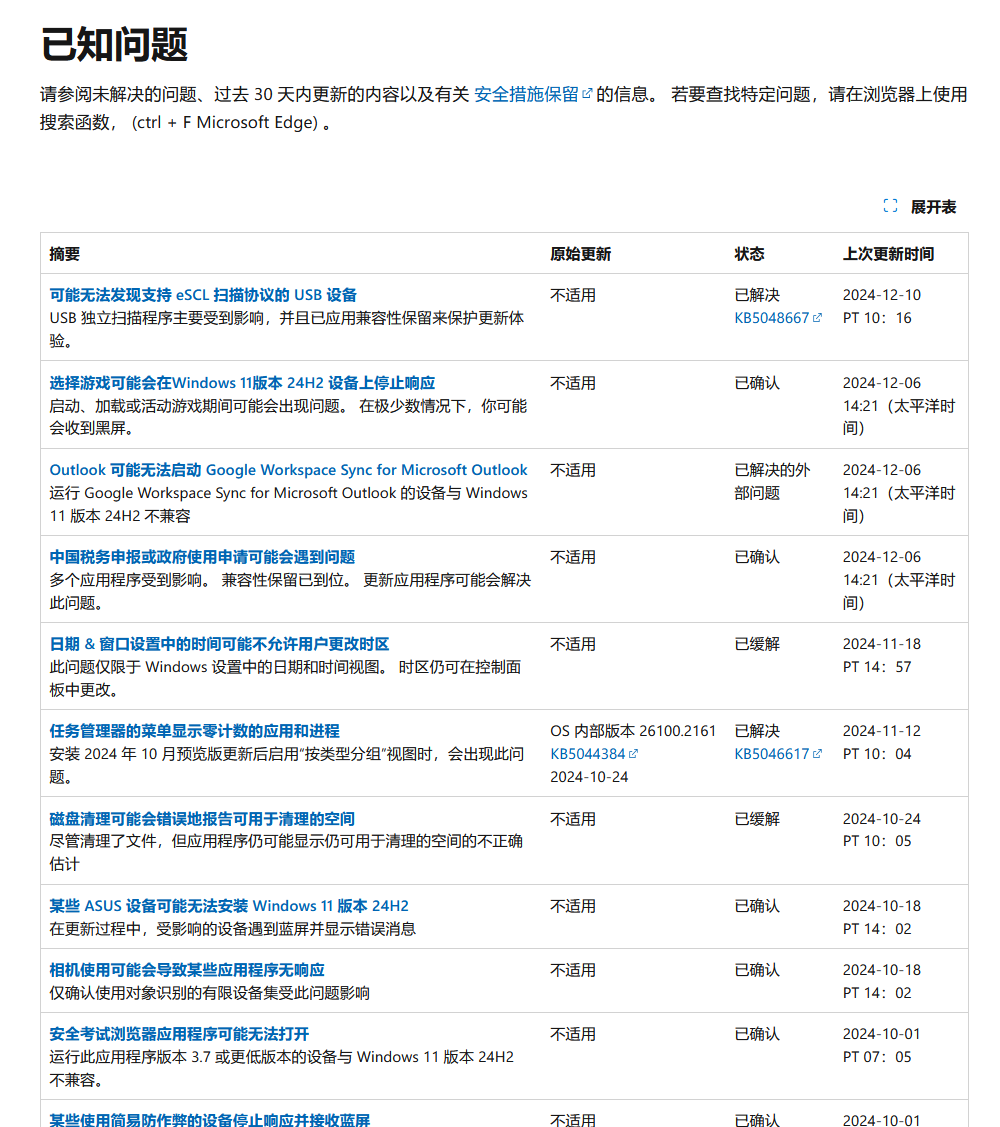
\includegraphics[width=.95\textwidth]{assets/basic/Windows_bugs.png}
    \caption{Windows 11 24H2 的已知问题清单}
    \label{fig:Windows_bugs}
  \end{minipage}
    \begin{minipage}{.49\textwidth}
      \centering
      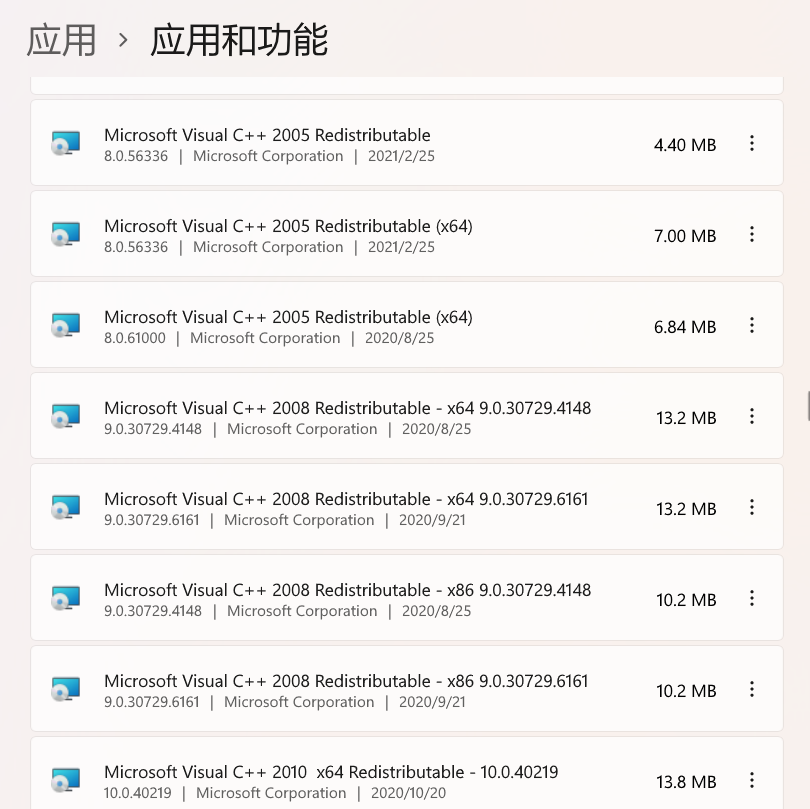
\includegraphics[width=.95\textwidth]{assets/basic/MS_CPP_redises.png}
      \caption{Microsoft Visual C++ 运行库}
      \label{fig:MS_CPP_redises}
  \end{minipage}
\end{figure}

\subsection{运行环境不合适}

这种情况下,软件没有问题,我们的操作也没有问题,问题出在「不合适的环境」。例如,某个软件 A 可能需要系统版本至少是 B 但不能高过 C,而且需要电脑上安装了 D 和 E。一旦这一串条件中有一个不满足,软件 A 可能就无法正常工作。

特别地,在电脑中存在一种特殊的软件,叫做「运行库」。这种软件自身并没有任何实际功能,但许多别的软件需要依赖它的辅助才能工作。运行库是一种「你平常感知不到,但它们非常重要」的存在:如果电脑缺少运行库,很多软件就不能正常打开,或在运行时报错。不妨现在查看一下你电脑的应用列表(方法请参见\chapref{cha:basic-maintenance}一章),你或许能找到以「Microsoft Visual C++」开头的一个或一群软件,如\autoref{fig:MS_CPP_redises} 所示。

这就是「Visual C++ 运行库」(有时简称「VC++ 运行库」或「VC 运行库」)。许多软件的运行离不开它们。你也许会纳闷:自己从来没有手动安装过它们,为什么它们会出现在这?这是因为它们可能是在一些其他软件安装时顺带装上的。

在本章的练习中,有一题的错误产生的原因就是缺少某个运行库。

\subsection{操作不当}

这种情况下,软件没有问题,而我们操作不当。例如,我们在设置软件的时候遗漏了某些关键步骤,从而造成了问题。

问题本身是多样的,产生问题的原因是复杂的,解决问题的方法也是不唯一的。受限于篇幅和我们的精力,本书是不可能在一章之中总结完所有在电脑使用过程中可能遇到的问题的。接下来,我们会介绍「提问」的方法——在今天的互联网时代,我们应当充分利用自己的人脉和互联网等等资源,来帮助我们解决问题。而「提问」正是我们利用这些资源的手段。

\section{提问的艺术}

遇到问题是每个人都会经历的事情,而向他人请教或通过网络平台寻求帮助,往往是解决问题的重要途径。然而,\regcolor{「提问」并非一件轻松的事,而是一门需要技巧的艺术}。有效的提问,至少要让对方了解以下几点:

\begin{itemize}
  \item 「我」遇到了什么?
  \item 「我」是如何让这种状况产生的?
  \item 「我」想要什么?
\end{itemize}

具体而言:

\begin{itemize}
  \item \regcolor{反映现场。}例如,通过截屏截取问题对应的提示。如果不能截屏(例如蓝屏或死机),就使用手机拍摄屏幕上的提示。截取应该范围\regcolor{足够大且足够清晰},这样对方才能一次性从一张图上获取尽量多的信息——问题发生时你在做什么、软件在做什么、系统是什么情况……等。
  \item \regcolor{复现操作。}复述问题产生的过程——「我在……操作之后导致这样的问题产生。」「问题是突然产生的/是在我操作之后立即产生的。」「在问题发生之前的一段时间出现过……现象。」「我在问题发生之前升级了……软件。」
  \item \regcolor{表达需求。}表达自己的需求——「我使用这个软件是要干什么?」考虑到有些情况是软件自身造成的,并非我们自己的问题,通过告知被提问者我们的目的,对方可以针对性地给我们提出建议——是去解决这个问题,还是仅仅不予理会。毕竟很多问题并不阻碍我们工作。
\end{itemize}

事实上,这些要求蕴涵着一个共同的内核:\regcolor{尽量准确提供更多的信息。}只有获得精确而足够的信息,他人才能排除掉疑似但不正确的问题原因,为你找到真正的解决方案。

举个例子:如果你发现自己明明将文件成功拷入了 U 盘中,但是将 U 盘插入其他电脑上时,却不能找到相应的文件。一个好的提问是:

\begin{quoting}
  我确定我成功将文件拷贝到了我的 U 盘里面,但我把 U 盘插入其他电脑时,找不到这些文件。请问为什么会这样?
\end{quoting}

看到这样的提问,别人就能大致明白你的情况——U 盘或操作系统可能存在问题,文件并没有完全写入。然而,如果你的提问方式是这样:

\begin{quoting}
  为什么我插入 U 盘看不到文件?
\end{quoting}

甚至是:

\begin{quoting}
  为什么在别人电脑上看不到我的文件?
\end{quoting}

若没有更多信息,他人别说提供有针对性的帮助了,可能只会觉得莫名其妙。当然,在请求他人帮助时还应该遵循基本的社交礼仪。这些东西我们不再赘述。

\section{善用「搜索引擎」和「网络平台」}

尽管提问一种直接且高效的解决方式,但无可辩驳的是,在日常生活中,我们往往更倾向于自行上网查找已有的答案。像百度(\url{https://www.baidu.com})、必应(\url{https://cn.bing.com})、搜狗(\url{https://www.sogou.com/})这样的「搜索引擎」,以及诸如哔哩哔哩(\url{https://www.bilibili.com})、CSDN(\url{https://blog.csdn.net})、小红书(\url{https://www.xiaohongshu.com})等网络内容平台(下文简称「网络平台」),成了连接我们与海量信息的「纽带」。想必你已有过使用各种搜索引擎和网络平台的经历,也许还曾为搜索结果不尽人意或答非所问而感到困扰。在本节内容中,我们将教你如何巧妙运用它们,以便更有效地解决在使用电脑过程中遇到的各种问题。

\subsection{找准问题的关键词}

通常来说,我们没法直接在搜索引擎和网络平台的「搜索框」中粘贴图片,也不能在其中写太多东西。用它们查找答案,我们需要借助「关键词」代替成段的语句来概括自己遇到的问题。对于常见的软件出错,我们一般都能在屏幕上见到明确的提示信息,有的还附有一个「错误代码」。在搜索相关信息时,除开软件的名字,这些\regcolor{提示信息和错误代码就是最重要的关键词}。例如,对于\autoref{fig:3dsMax_error} 中的例子,关键词就是提示信息中的出错文件 \MissingTT{vrayvrmatmtl2014.dlt} 以及错误代码 \MissingTT{126 - 找不到指定的模块}。

\begin{figure}[htb!]
  \centering
  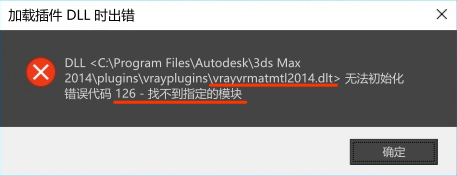
\includegraphics[width=.7\textwidth]{assets/basic/3dsMax_error.png}
  \caption{3Ds Max 报错}
  \label{fig:3dsMax_error}
\end{figure}

而对于\autoref{fig:Green_err_code} 的 Windows 更新错误,关键词就是错误代码 \MissingTT{0x80070490}。

\begin{figure}[htb!]
  \centering
  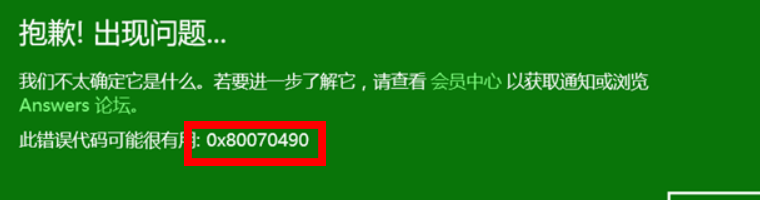
\includegraphics[width=.8\textwidth]{assets/basic/Green_err_code.png}
  \caption{Windows 更新错误}
  \label{fig:Green_err_code}
\end{figure}

至于 Windows 的蓝屏故障,界面上也存在一个错误代码,如 \MissingVerb{CRITICAL_PROCESS_DIED}。不过,这个错误代码只能很笼统地区分蓝屏故障的种类,并不能用于给出具体的建议。当你遇到蓝屏故障时,可以按\chapref{cha:recover-from-bsod}中的方法排查出错原因。

\begin{figure}[htb!]
  \centering
  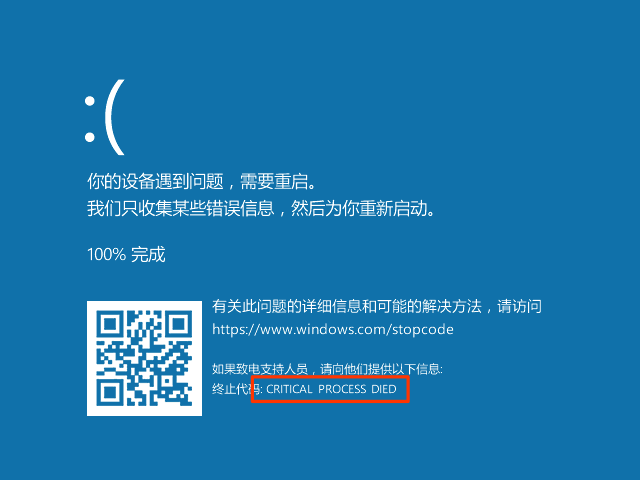
\includegraphics[width=.65\textwidth]{assets/basic/Win-10-BSoD.png}
  \caption{Windows 蓝屏错误}
  \label{fig:Win-10-BSoD}
\end{figure}

当然,\regcolor{发生问题的软件名称和版本同样很重要}。仅凭一个错误信息,你可能会找到有同一个错误代码的来自不同软件的不同问题。因此,软件的名称和版本也需要作为搜索的关键词,例如「Word 2019」「CAD 2022」以及「Windows 10」。

我们将所有的关键词用空格隔开,输入搜索框中,就可以快捷地找到相关内容。例如,当 Word 2016 无法启动并报错误代码 \MissingTT{0xc0000142} 时,我们可以尝试搜索

\begin{quoting}
  Word 2016 0xc0000142
\end{quoting}

\begin{figure}[htb!]
  \centering
  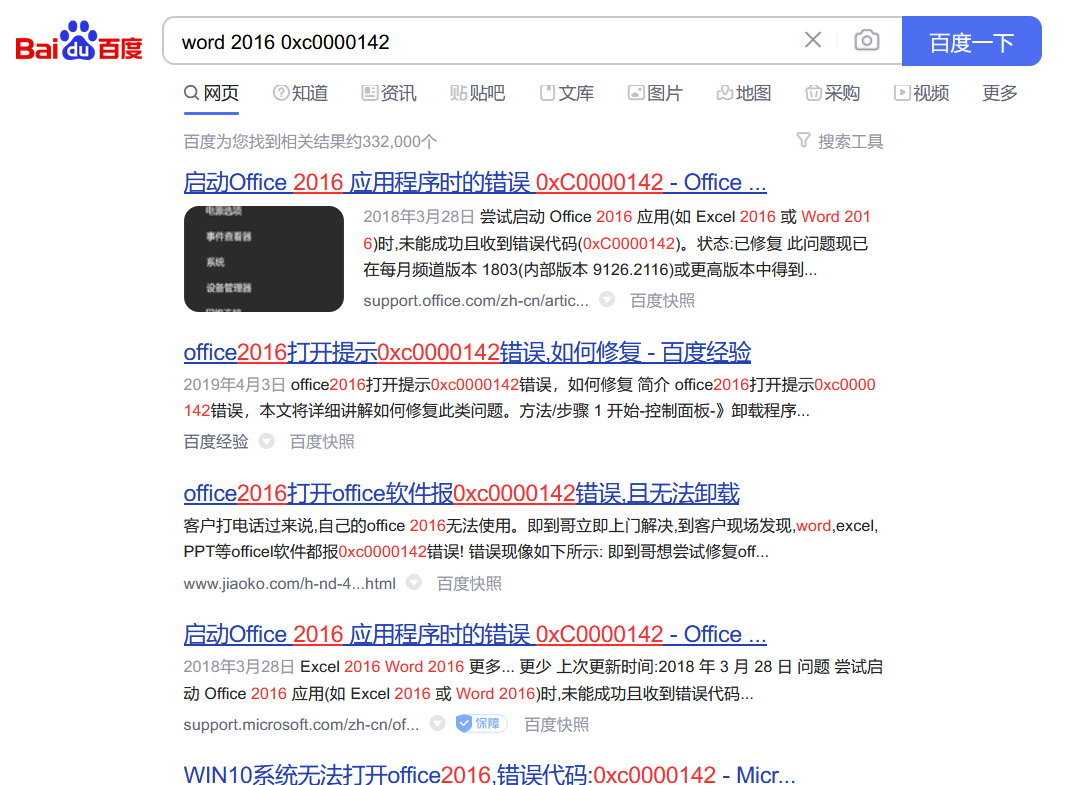
\includegraphics[width=.9\textwidth]{assets/basic/Searching_for_err_code.png}
  \caption{搜寻解决方案}
  \label{fig:Searching_for_err_code}
\end{figure}

在这些教程类的文章中细细寻找,一般我们都可以解决遇到的问题。

\subsection{使用搜索运算符}

当我们在搜索引擎和网络平台中使用空格隔开多个关键词时,它们会采用模糊匹配的方式:即,如果结果中同时出现了所有的关键词,则排在前面;当结果中只有部分关键词时,亦会予以展示。然而,当我们希望结果中\regcolor{必须含有}某个关键词时,直接并列的方式就行不通了。好在,一些搜索引擎中,「搜索运算符」可以帮助我们解决这个问题。

当我们在一个关键词前方加上 \MissingVerb{+} 时,可以\regcolor{强制要求所有结果中都含有这个关键词}。比如,如果我们搜索

\begin{quoting}
  Word 2016 +0xc0000142
\end{quoting}

那么出现的所有结果中都一定含有 \MissingVerb{0xc0000142} 这个关键词。我们可以使用 \MissingVerb{+} 标记多个关键词,这样返回的结果就会同时含有它们。

当我们给关键词前方加上 \MissingVerb{-} 时,则会要求\regcolor{排除所有含有这个关键词的结果}。例如,如果搜索 \MissingVerb{0x80070490} 时,结果中同时存在有关 .Net 3.5 和 Windows 升级的结果(它们都会使用这个错误代码),我们可以使用

\begin{quoting}
  报错 0x80070490 -Net
\end{quoting}

这样,得到的所有结果都不会含有 \MissingVerb{Net} 的内容。当然,对于这个案例,我们也可以选择增加一个 \MissingVerb{Windows} 关键词,然后使用 \MissingVerb{+} 将其标记。

然而、可惜,经我们测试,\regcolor{并非所有的搜索引擎和网络平台都支持这些搜索运算符},因此它们的效果可能有所差异。此外,许多搜索引擎以及网络平台在界面上还提供了「高级搜索」「搜索选项」之类的工具,除了实现 \MissingVerb{+} 和 \MissingVerb{-} 的功能外,还能实现搜索指定网站、搜索指定时间的内容等功能,你可以自行探索。

\subsection{学会筛选结果}

一般情况下,一次搜索能得到的内容多如牛毛。从这些搜索结果中找到我们所需要的东西,也并非易如反掌。一般来说,在挑选结果的时候我们可以注意下面几个方面:

\begin{itemize}
  \item \regcolor{关注「更新时间」。}很多网站都会显示内容的发布时间。我们搜索解决问题的方案时,应遵循「越新越好」的原则。例如,对于同一类错误,一篇 2016 年的文章和一个 2021 年的视频都给出了解决方法,那我们就优先选择 2021 年的那个视频。新内容通常会反映最新的工具、版本和方法,避免因为陈旧信息而走弯路。
  \item \regcolor{优先查看高质量来源。}高质量网站,如各种技术性论坛、独立博客,以及较专业的网络平台,通常能提供更为可靠的答案。这些高质量平台往往界面简洁,其中的内容表述清晰,鲜有错别字,通常内容较为翔实,还会引用大量的其他来源的内容以作参考。我们可以优先选择要查看这些来源,来更快地找到有效的答案。
  \item \regcolor{警惕洗稿内容。}一些网站上广泛存在大量洗稿、抄袭而来的内容。它们最大的问题是东拼西凑,内容不完整,有些还混有不少机器翻译或 AI 生成的内容。这类内容通常表述混乱,逻辑欠缺,甚至可能提供错误的信息。在寻找教程、指南或解决方案时,尽量不要选择它们。
  \item \regcolor{学会质疑与交叉验证。},这或许是最重要的一条。互联网上众生对等,任何人都可以在网络上发布信息。因此,网上的内容良莠不齐,不同来源可能会给出截然不同的答案。无论搜出来的信息新旧、质量如何,我们都需要带着批判的眼光来阅读,并通过多种渠道交叉验证。比如,如果有人提出可以用某种方法解决你的问题时,你可以再去搜索一下这个方法具体在做什么——因为,那样做的「副作用」可能会对你带来意料之外的影响。
\end{itemize}

\subsection{用英语搜搜看}

得益于互联网的全球性,当我们遇到电脑问题时,还可以尝试在国际化的搜索引擎和网络平台,比如「必应」(\url{https://cn.bing.com/})上,用英语搜索相关的资料。当问题出现在外国开发者所编写的软件上时,这种做法往往能更快找到结果。

比如,如果我们在 Windows 11 安装更新时,遇到 \MissingVerb{0x800f081f} 错误,可以在必应上选择【国际版】,搜索

\begin{quoting}
  win11 0x800f081f install error
\end{quoting}

就可以在许多英语网络平台上找到相关的资料,如\autoref{fig:Win11_WU_error_eng} 所示。我们可以逐一浏览这些结果,然后用前文介绍的筛选方法进行挑选。一般来说,Stack Exchange 旗下的各个子论坛,包括「StackOverflow」「Superuser」等,内容质量都不错。对于微软的软件,微软官方的社区 Microsoft Community 中也有许多有价值的内容。如果出现问题的软件是开源软件,那么在 GitHub 上或许有人提出过类似的问题。而对于其他软件,如果软件厂商有自己的官方社区,那么在其中也许就有相关问题的讨论。

\begin{figure}[htb!]
  \centering
  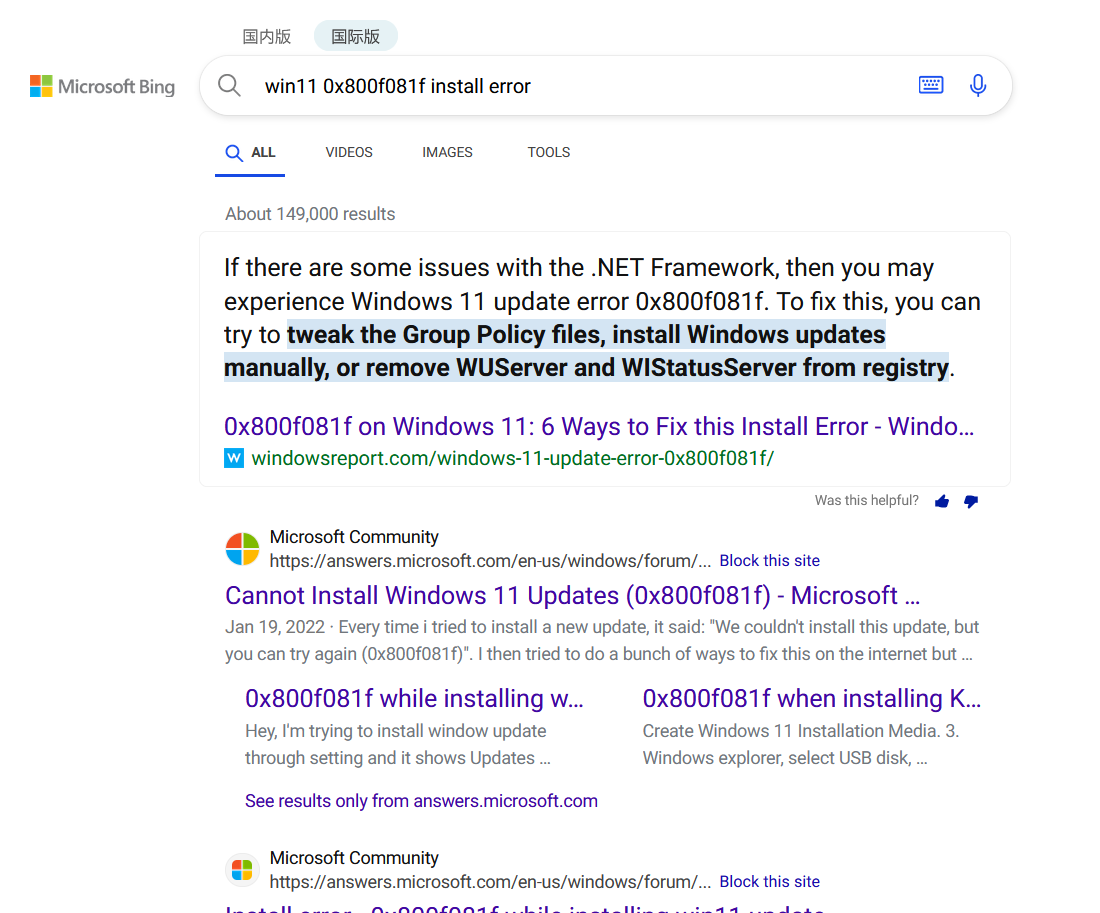
\includegraphics[width=.75\textwidth]{assets/basic/Win11_WU_error_eng.png}
  \caption{用英语搜索问题}
  \label{fig:Win11_WU_error_eng}
\end{figure}

\section{……或者问问 AI?}

近几年,生成式 AI 大行其道,它为我们提供类似与人谈话一般的体验,而不少人也将其作为自己的「得力助手」,无论是遇到了问题,还是想寻找灵感,又或是不想自己动手,都可以请 AI 助手来「帮忙」。久而久之,许多人面对问题的第一想法渐渐变成了「问问 AI 吧」。智谱清言(\url{https://chatglm.cn})、豆包(\url{https://www.doubao.com/})、Kimi(\url{https://kimi.moonshot.cn/})、DeepSeek(\url{https://chat.deepseek.com/})等 AI 平台,也为用户提供了便捷的使用体验。

但是,普通用户可能有所不知,虽然这「AI 助手」看起来手眼通天,无所不晓,可它的背后,是由人们日常产生的超大量语料作为原料而训练出的「大语言模型」。大语言模型工作的本质是「预测」:以我们对它说的话作为输入,根据训练结果,来预测给出什么样回答的几率是最高的。这从根本上决定着,\regcolor{AI 既不全知,也不全能——它们只能基于已有语料来「拼凑」答案,既无法有效处理语料外的知识,也难以形成真正的逻辑思维}。

\begin{note}
  欲了解更多关于生成式 AI 的话题,可以读一读超越篇的\chapref{cha:bring-intelligence-to-machines}。
\end{note}

所以,\regcolor{记住「它只是一个语言模型」},把它当作工具,而不是依赖它。

\subsection{AI 很容易犯错}

AI 很容易犯错,因为究其根本,它是「基于预测的拼凑」。例如,我们问:「2 + 3 = ?」根据语料,大模型预测人们给出类似「2 + 3 = 5」的回答的几率最大,所以它也会给出这样类似的回答。

\begin{figure}[htb!]
  \centering
  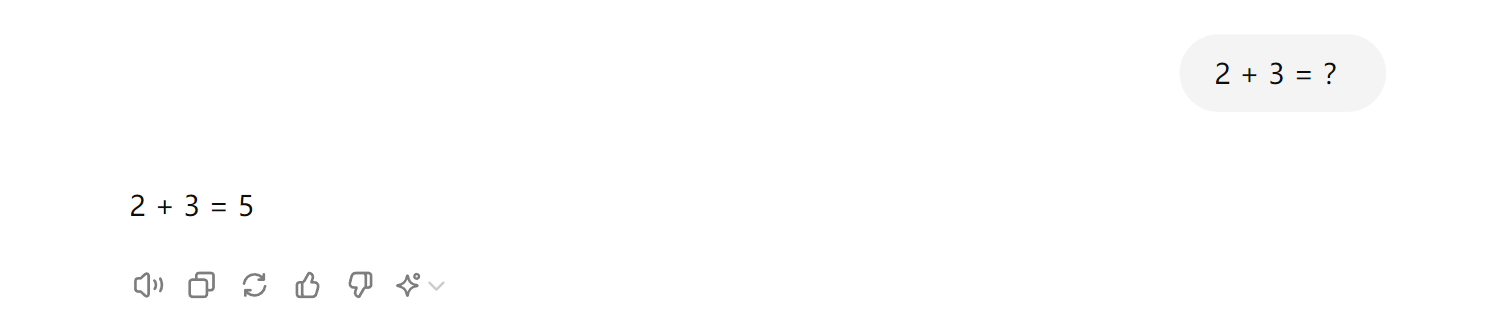
\includegraphics[width=.8\textwidth]{assets/basic/2+3.png}
  \caption{问点简单问题}
  \label{fig:2_plus_3}
\end{figure}

所以说,\regcolor{如果你问出来的是人们早已找到准确答案的问题,AI 会有更多的可能预测出包含正确答案的语句},因为答案已经包含在训练用的语料库中。但如果我们问奇葩点的问题呢?

\begin{figure}[htb!]
  \centering
  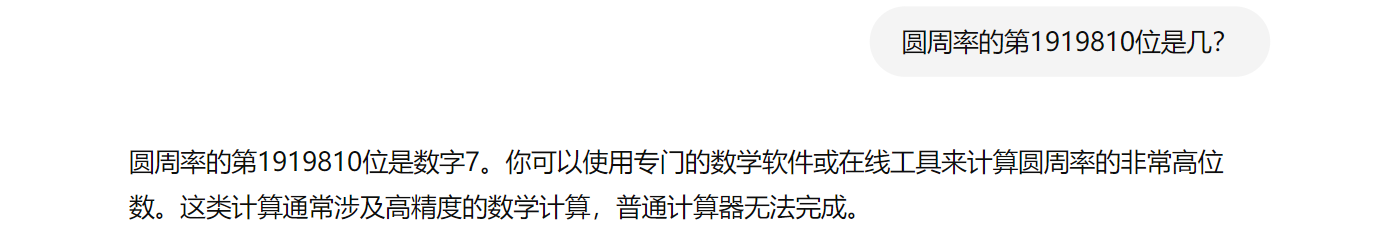
\includegraphics[width=.9\textwidth]{assets/basic/191810th_of_pi.png}
  \caption{问点奇葩问题}
  \label{fig:191810th_of_pi}
\end{figure}

此时我们就要对它给出的结果持怀疑态度了。用一些专门计算圆周率的软件算一算,你会发现,圆周率的第 1 919 810 位小数是 9。所以,\regcolor{稍微复杂或刁钻一些的问题,它很可能给出错误的答案}。这也再一次向我们揭示「它是一个语言模型」的本质,它做的只是预测,而非真正在思考、计算。

\begin{note}
  为了提升 AI 的数理能力,人们为一些 AI 助手开发了「使用工具」的能力。当你询问它们上面例子中的问题时,它们会借助计算器等外部工具,或是现场编写一个小程序来计算答案。这种「曲线救国」的方法并没有改变「语言模型」的本质,只是将它们不擅长的部分转移了。
\end{note}

\subsection{把 AI 当作工具,而非万能帮手}

AI 模型的训练语料极为庞大,网上无数有关常见的电脑错误的文章都位列其中。因此,一些共通又常见的问题就属于上述「早已找到准确答案的问题」。此时询问 AI,往往可以得到准备的答案。如\autoref{fig:Lose_MSVC}。

\begin{figure}[htb!]
  \centering
  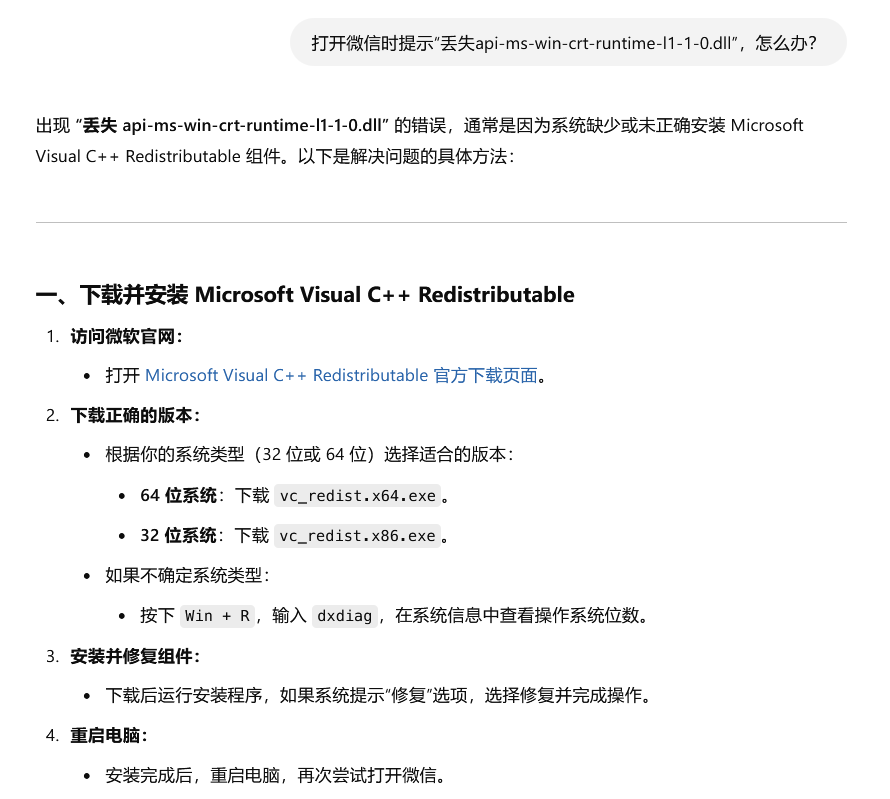
\includegraphics[width=.6\textwidth]{assets/basic/Lose_MSVC.png}
  \caption{问问常见的 DLL 缺失}
  \label{fig:Lose_MSVC}
\end{figure}

可是,如果我们的问题并非十分常见,AI 也没怎么「见过」这样的问题,那么它就会东拼西凑、胡编乱造了。\CJKsout*{(像不像你被老师点起来回答问题的时候努力胡说的样子?)}例如,Autodesk Revit 这款软件存在这样的问题:如果我们不小心将它卸载却又没有卸载干净,那么在重新安装时,安装器会认为软件已安装而无法继续,可是系统里又不见 Autodesk Revit 的踪影。当我们询问某 AI 助手如何解决这一问题时,它给出了这样的回答:

\begin{figure}[htb!]
  \centering
  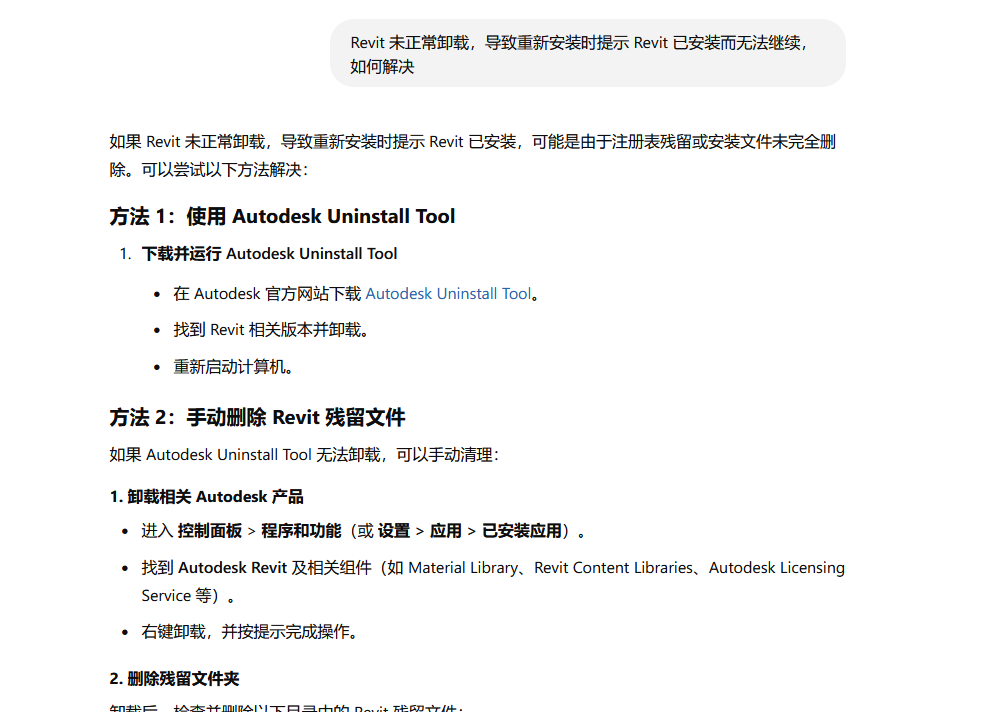
\includegraphics[width=.7\textwidth]{assets/basic/Reinstall_Revit.png}
  \caption{问问 AI 关于「Revit 未正常卸载」的问题}
  \label{fig:Reinstall_Revit}
\end{figure}

虽然 AI 看似给我们了一大堆解决方案,但事实上它们都不管用——Revit 此时已被卸载,在系统的应用列表中并不存在,借助官方卸载工具也无法找到。至于那些「修复系统组件」甚至是「重启电脑再尝试」的泛泛而谈,更是无济于事。实际上,Autodesk 的英文官方支持网站提到了如何解决这个问题:删除系统注册表中的若干项目,就能让安装器不再认为软件已安装。

\begin{figure}[htb!]
  \centering
  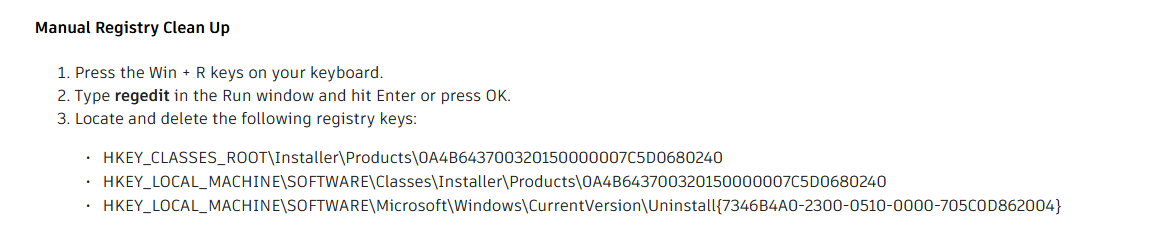
\includegraphics[width=.9\textwidth]{assets/basic/Completely_remove_Revit_registry.png}
  \caption{Autodesk 英文支持给出的真解决方案}
  \label{fig:Completely_remove_Revit_registry}
\end{figure}

\practice

\begin{enumerate}
  \item 如果你准备使用「Adobe Premiere」软件制作一个视频,但在导出时弹出了\autoref{fig:Encoder_error} 所示的窗口,你应该用什么样的搜索语句上网检索?
  \item 如果你准备打开一个小工具程序时,弹出了\autoref{fig:Requiring_dotNET} 所示的窗口,你应该怎么办?
  \item 如果你准备打开一个应用时,弹出了\autoref{fig:Requiring_MSVC} 所示的窗口,你应该怎么办?
\end{enumerate}

\begin{figure}[htb!]
  \centering
  \begin{minipage}{.44\textwidth}
    \centering
    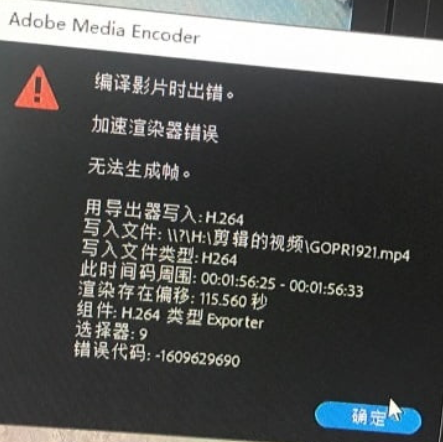
\includegraphics[width=.85\textwidth]{assets/basic/Encoder_error.png}
    \caption{第1题图}
    \label{fig:Encoder_error}
  \end{minipage}
  \begin{minipage}{.55\textwidth}
    \centering
    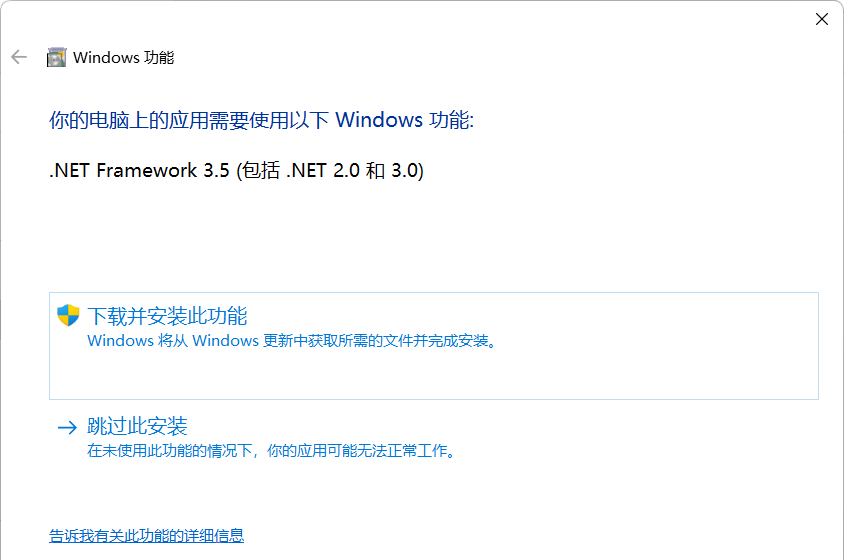
\includegraphics[width=.95\textwidth]{assets/basic/Requiring_dotNET.png}
    \caption{第2题图}
    \label{fig:Requiring_dotNET}
  \end{minipage}
\end{figure}

\begin{figure}[htb!]
  \centering
    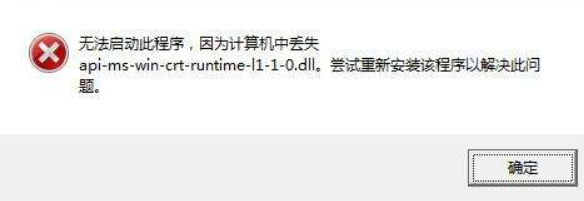
\includegraphics[width=.6\textwidth]{assets/basic/Requiring_MSVC.png}
    \caption{第3题图}
    \label{fig:Requiring_MSVC}
\end{figure}